\documentclass[a4paper,12pt]{article}
%\usepackage[latin1]{inputenc}
\usepackage[spanish]{babel}
\usepackage{graphicx}
\usepackage{amsmath}
\usepackage{hyperref}
\usepackage{xcolor}
\decimalpoint % El paquete \usepackage[spanish]{babel} tiene la coma por defecto como separador decimal... 

%\usepackage{wrapfig}
\setlength{\textheight}{250mm}
\setlength{\textwidth}{165mm}
\setlength{\topmargin}{-15mm}
\setlength{\oddsidemargin}{0pt}
\pagestyle{empty}
\usepackage[spanish]{cleveref}

\begin{document}

\def\bm#1{{\mbox{\boldmath $#1$}}}
\def\eqdef{\buildrel \rm def \over =}
\def\signo{\mathop{\rm signo}\nolimits}

\mbox{}\vspace*{-20mm}

{\centering
{\small\sc Escuela Técnica Superior de Ingenieros de Caminos, Canales y Puertos (Madrid)}\\*[4mm]
{\Large\bf Método de los Elementos Finitos (Curso 2021-22)}\\*[4mm]
Ejercicio 7. Cálculo dinámico \\*[4mm]
}

% \vspace{4mm}

\noindent
Se considera un pórtico plano representativo de la estructura de un edificio, que corresponde a una dimensión en dirección normal al plano de 3 m, y con el resto del dimensiones indicadas en la \cref{fig:croquis} adjunta. El material de este pórtico es elástico lineal con propiedades mecánicas $\text{E}=30$ GPa, $\nu=0.25$ y $\rho=2500$ kg/m$^3$. Se quiere estudiar el comportamiento dinámico de la estructura al estar sometida a una carga de viento lateral en el contorno $\overline{\text{AB}}$. Esta carga tiene una distribución parabólica de ecuación $y=22x^2$, alcanzando un valor máximo de 450 N/m$^2$ en la parte más alta de la edificación. La variación de esta carga en el tiempo se representa mediante una función sinusoidal con las parámetros mostrados en la \cref{fig:amplitud}.

Las columnas tienen una sección de $40 \times 40$ cm y las vigas horizontales una sección de $80 \times 20$ cm.

El modelo se realizará con elementos tipo viga lineales de Timoshenko (B21) y se discretizará con un tamaño aproximado de elemento de 0.7 metros. 
\vspace{5mm}

\begin{figure}[hb]
\begin{minipage}[b]{0.65\linewidth}
    \centering
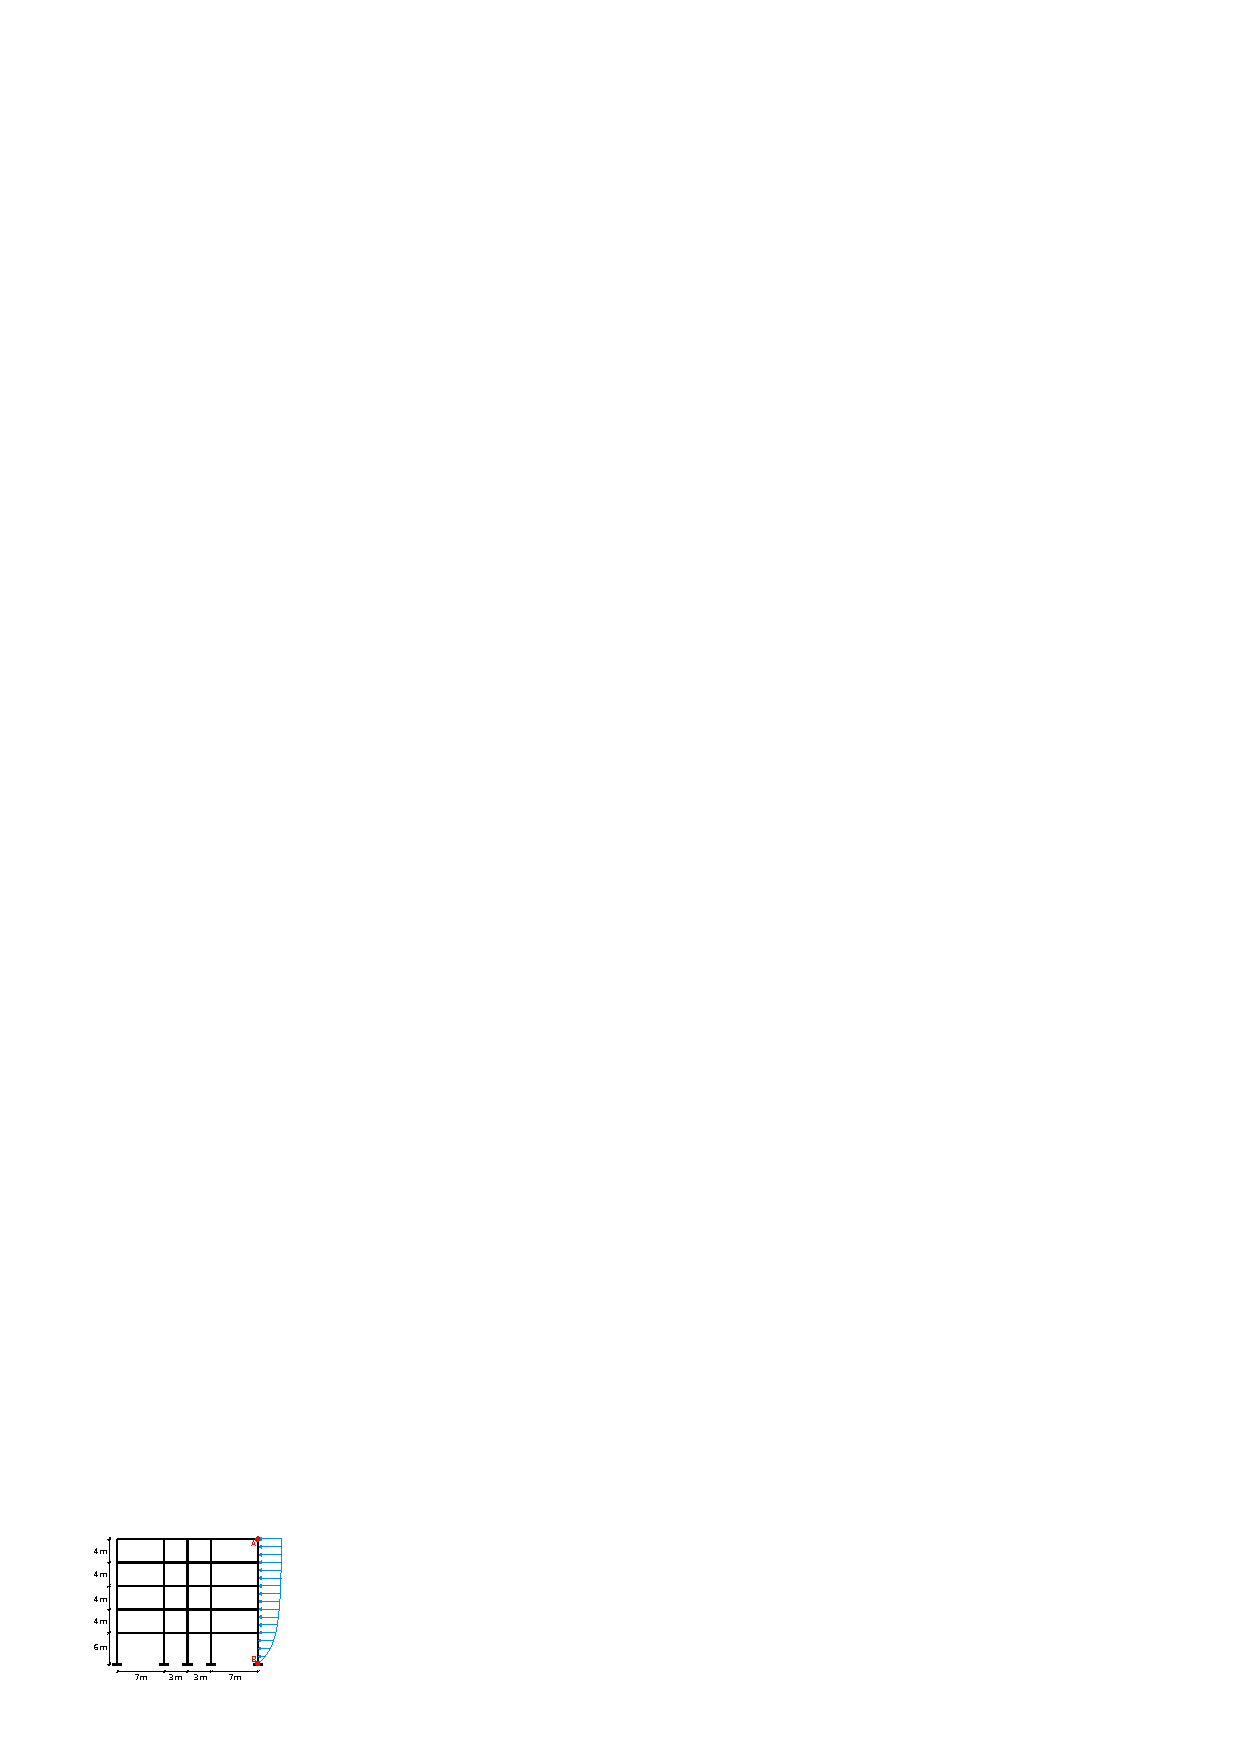
\includegraphics[width=\textwidth]{recorte}
\caption{Croquis de la edificación}
\label{fig:croquis}
\end{minipage}
\hspace{0.9cm}
\begin{minipage}[b]{0.25\linewidth}
    \centering
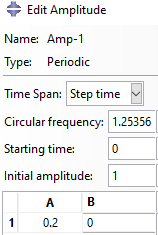
\includegraphics[width=\textwidth]{amplitud.png}
\caption{Amplitud}
\label{fig:amplitud}
\end{minipage}
\end{figure}

Se pide en primer lugar obtener los 5 primeros modos de vibración de la estructura. Posteriormente, se pide obtener la evolución del desplazamiento horizontal del nodo \textcolor{red}{A} y la evolución de la componente vertical de la reacción en el nodo \textcolor{red}{B} (durante 20 segundos de simulación) para los siguientes casos:

\begin{itemize}

    \item Realizando un cálculo con integración directa en el tiempo usando HHT con $\alpha_f=-0.33$ y con amortiguamiento de tipo Rayleigh de coeficientes $\alpha=0.861694$ y $\beta=0.000909$. Para este cálculo se utilizarán un máximo número de incrementos de tiempo de 10000 y un incremento de tiempo de 0.01 s
    \item Realizando un cálculo de análisis modal, considerando los 5 primeros modos de vibración, un incremento de tiempo de 0.1 s y un amortiguamiento modal de $3 \%$ para los modos 1, 2 y 3.

\end{itemize}

\end{document}

